\documentclass[titlepage]{article}
\usepackage{graphicx}
\usepackage{wrapfig}
\usepackage{enumitem}% http://ctan.org/pkg/enumitem
\graphicspath{ {./img/} }

\author{Jeffrey Meyer & Bayli Boston}
\title{Theory of Computer Sciece: Homework \#2 - NandToTetris}

\begin{document}

\maketitle

\newpage

\section{Project 1}

\begin{description}
  \item[And]{
    All test passed

    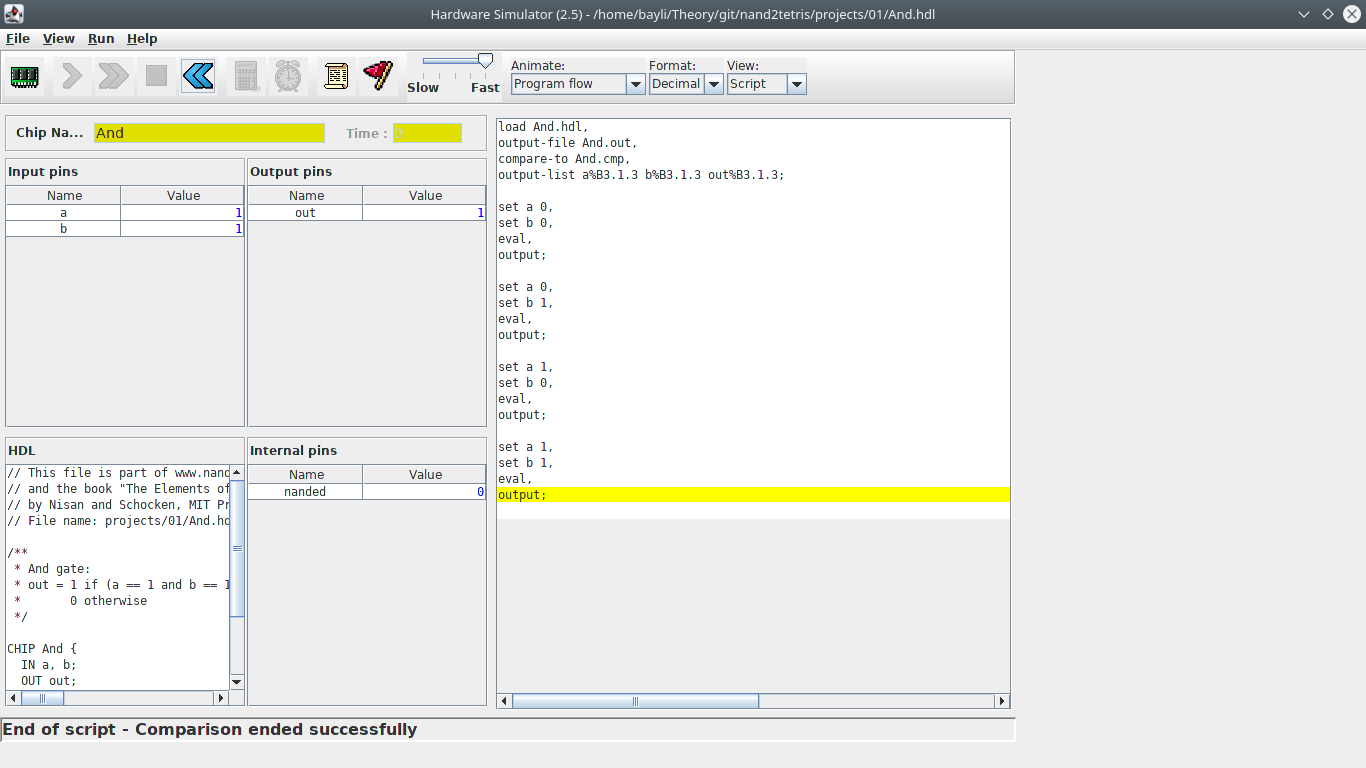
\includegraphics[width=.9\textwidth]{01/And.png}
  }
  \item[And16]{
    All test passed

    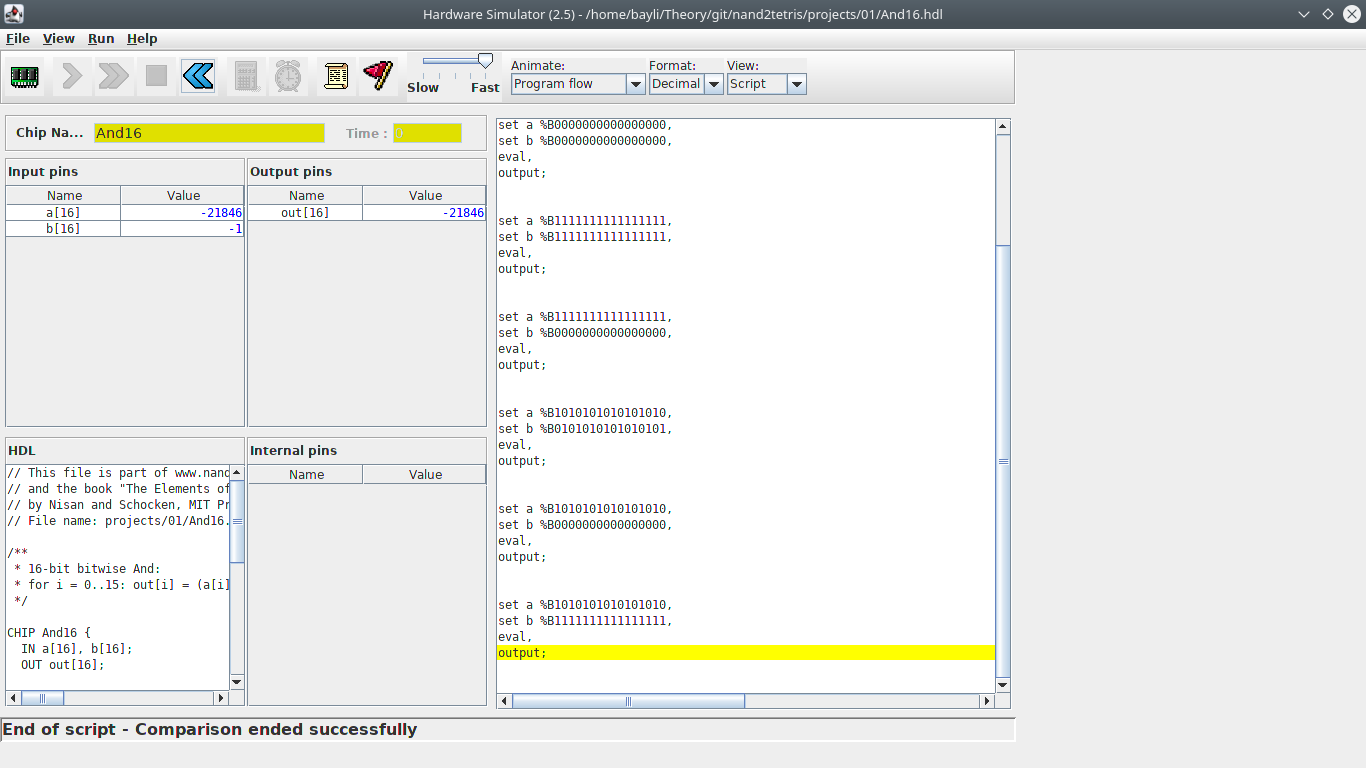
\includegraphics[width=.9\textwidth]{01/And16.png}
  }
  \item[DMux]{
    All test passed

    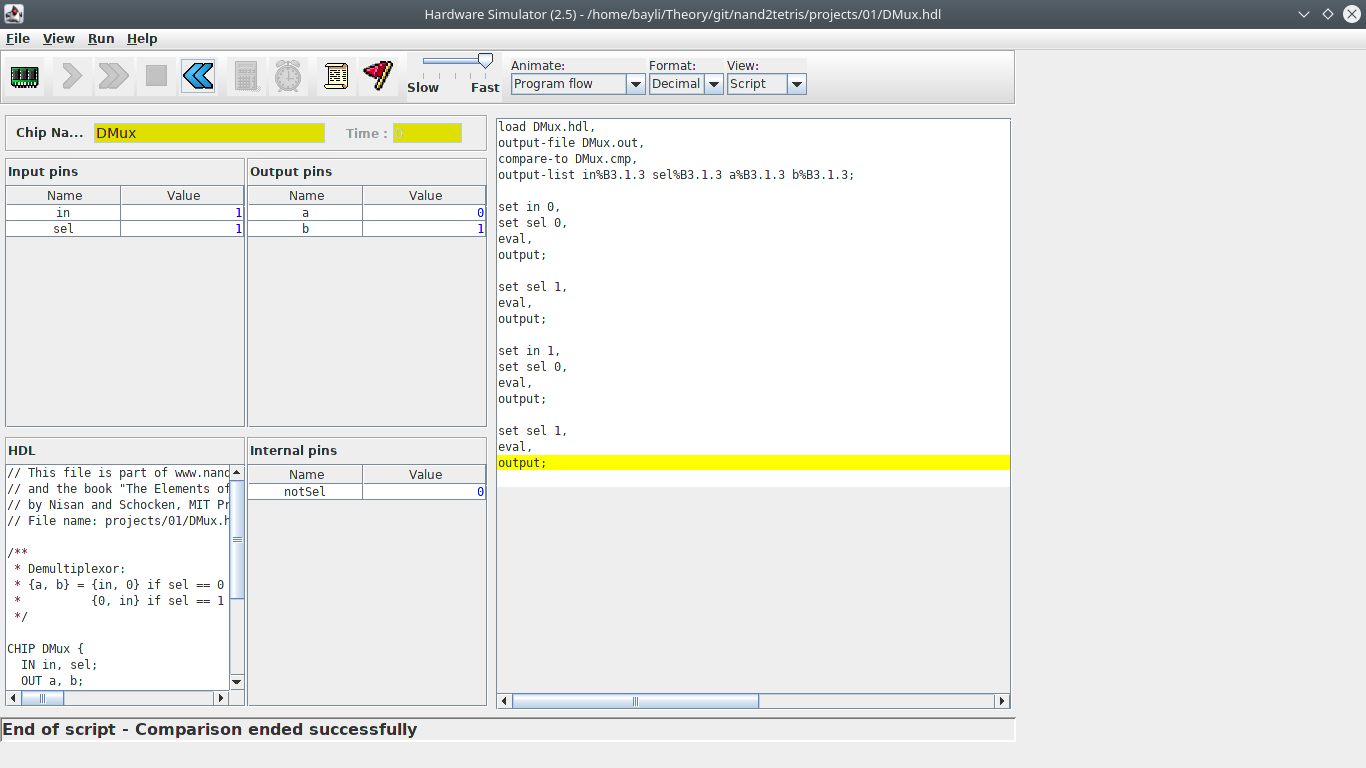
\includegraphics[width=.9\textwidth]{01/DMux.png}
  }
  \item[DMux4Way]{
    All test passed

    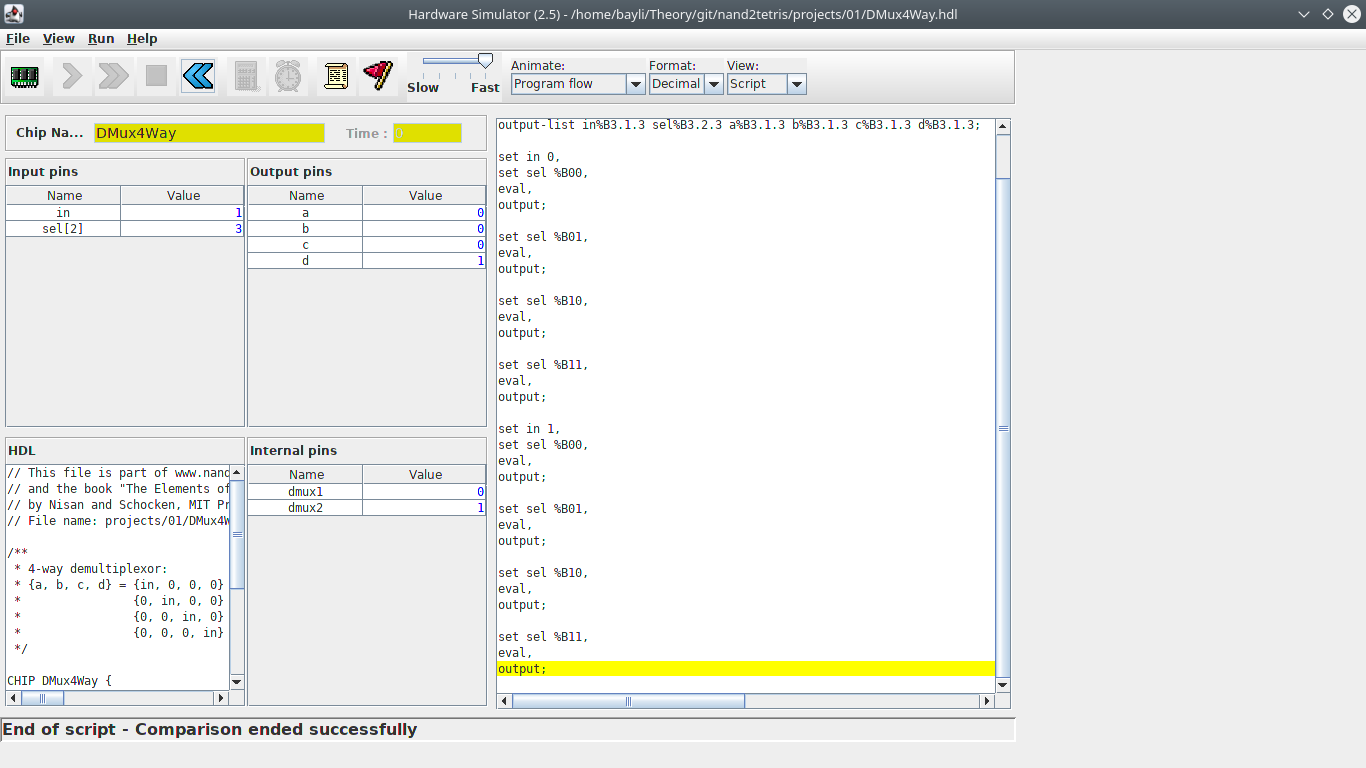
\includegraphics[width=.9\textwidth]{01/DMux4Way.png}
  }
  \item[DMux8Way]{
    All test passed

    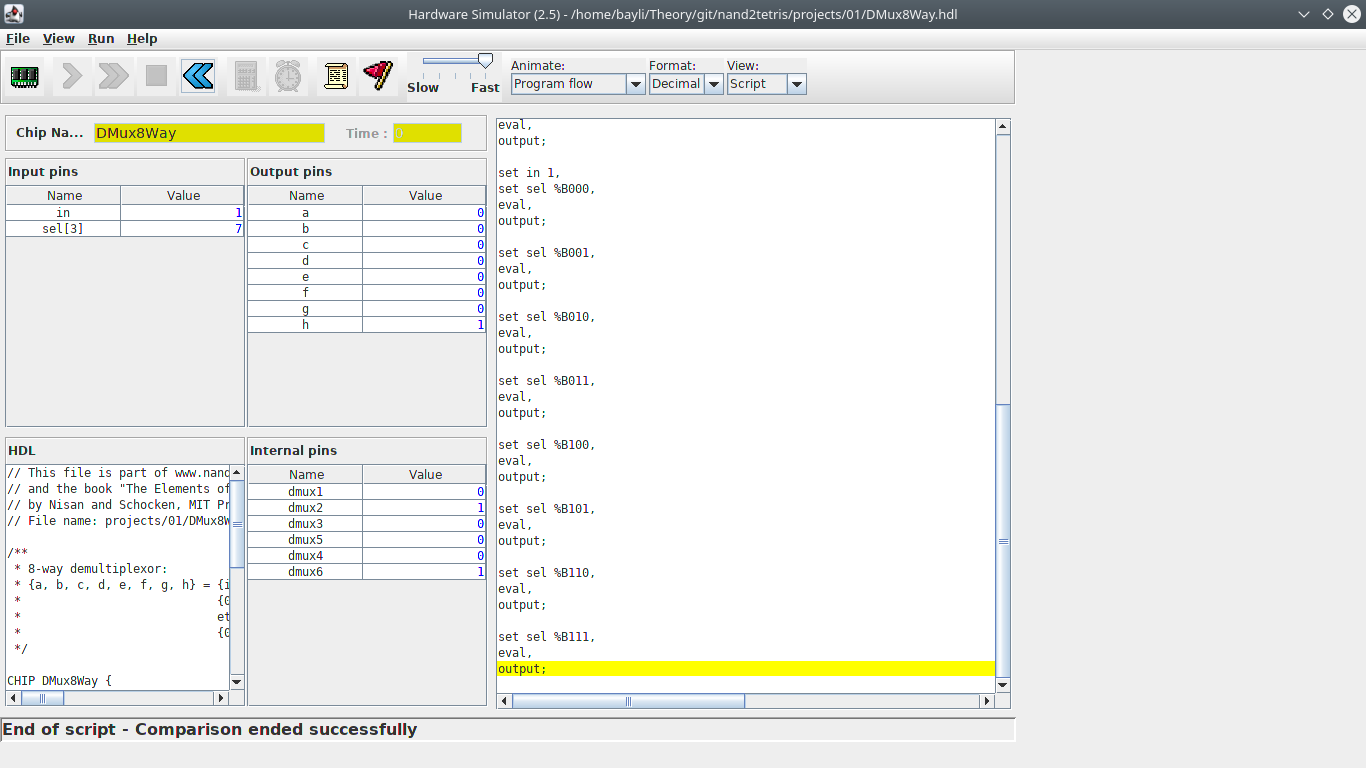
\includegraphics[width=.9\textwidth]{01/DMux8Way.png}
  }
  \item[Mux]{
    All test passed

    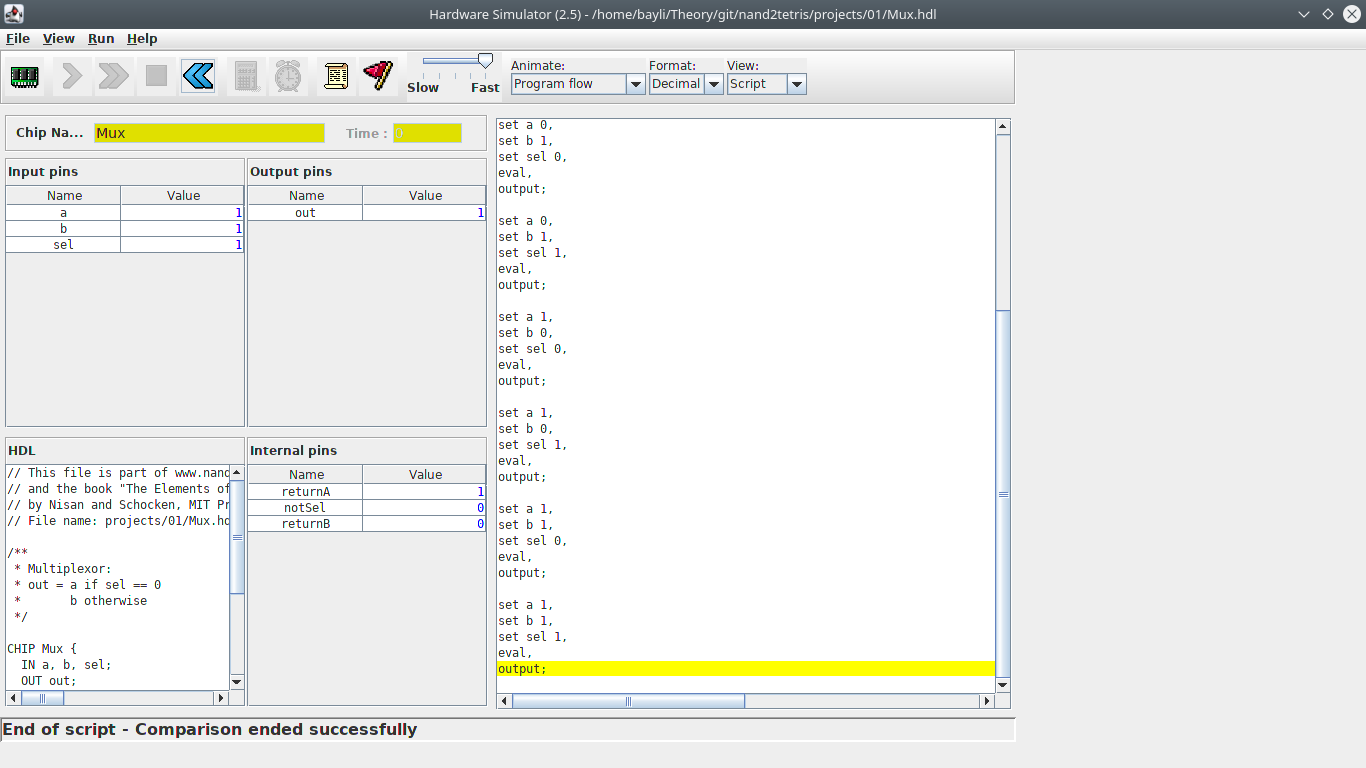
\includegraphics[width=.9\textwidth]{01/Mux.png}
  }
  \item[Mux4Way16]{
    All test passed

    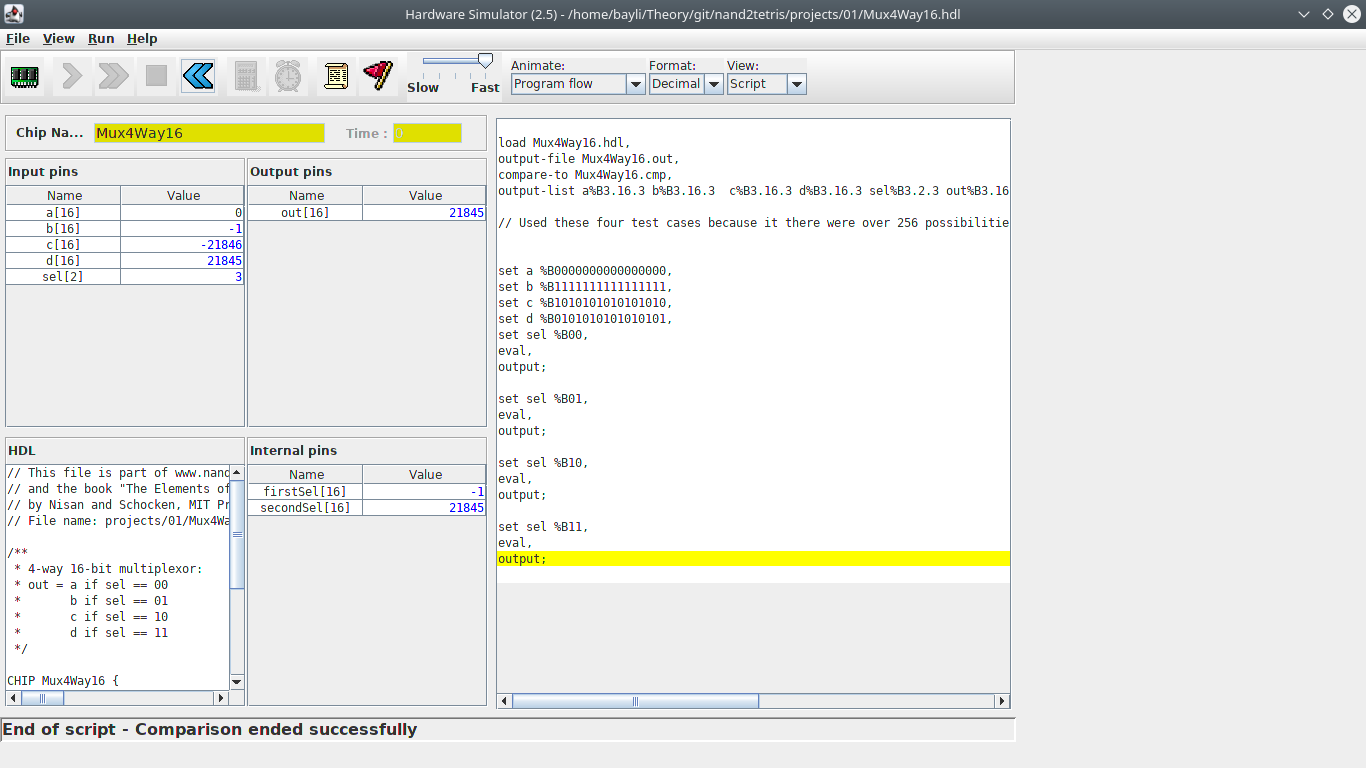
\includegraphics[width=.9\textwidth]{01/Mux4Way16.png}
  }
  \item[Mux8Way16]{
    All test passed

    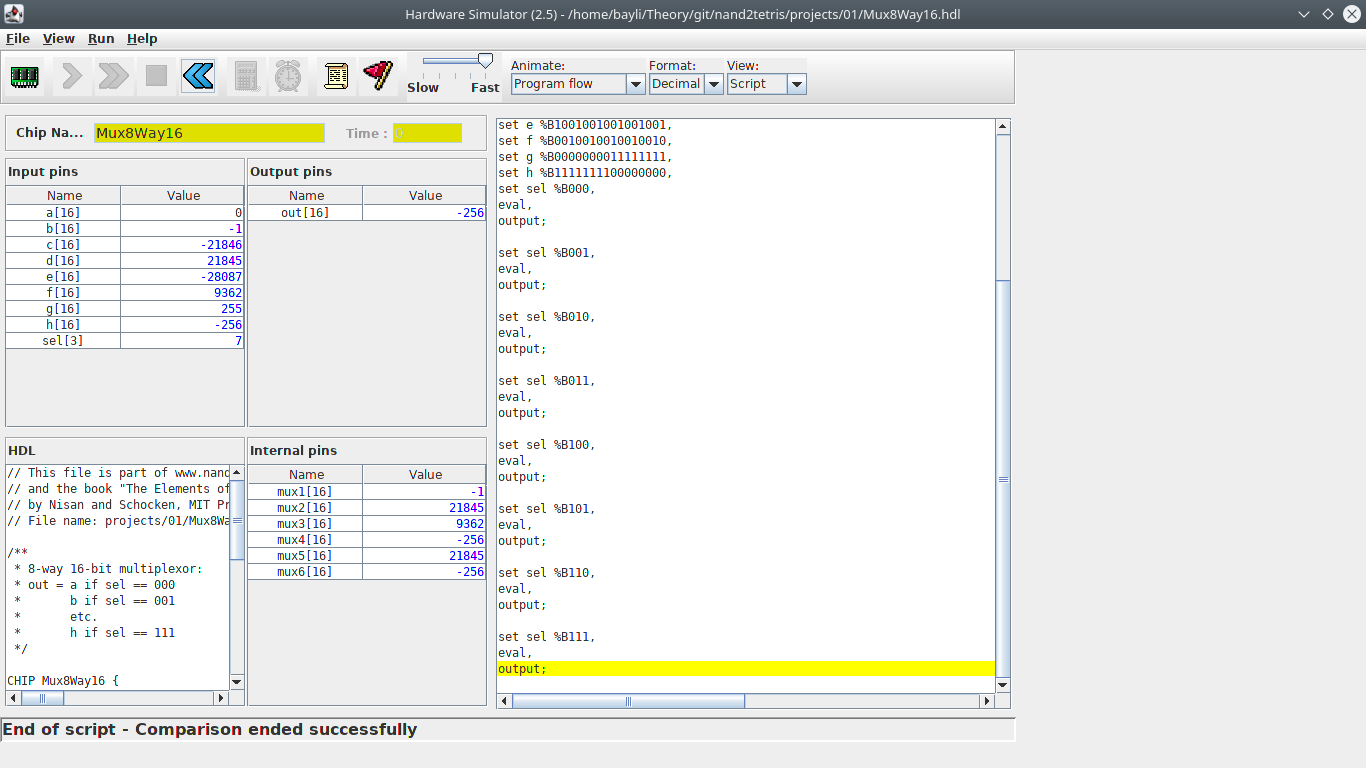
\includegraphics[width=.9\textwidth]{01/Mux8Way16.png}
  }
  \item[Mux16]{
    All test passed

    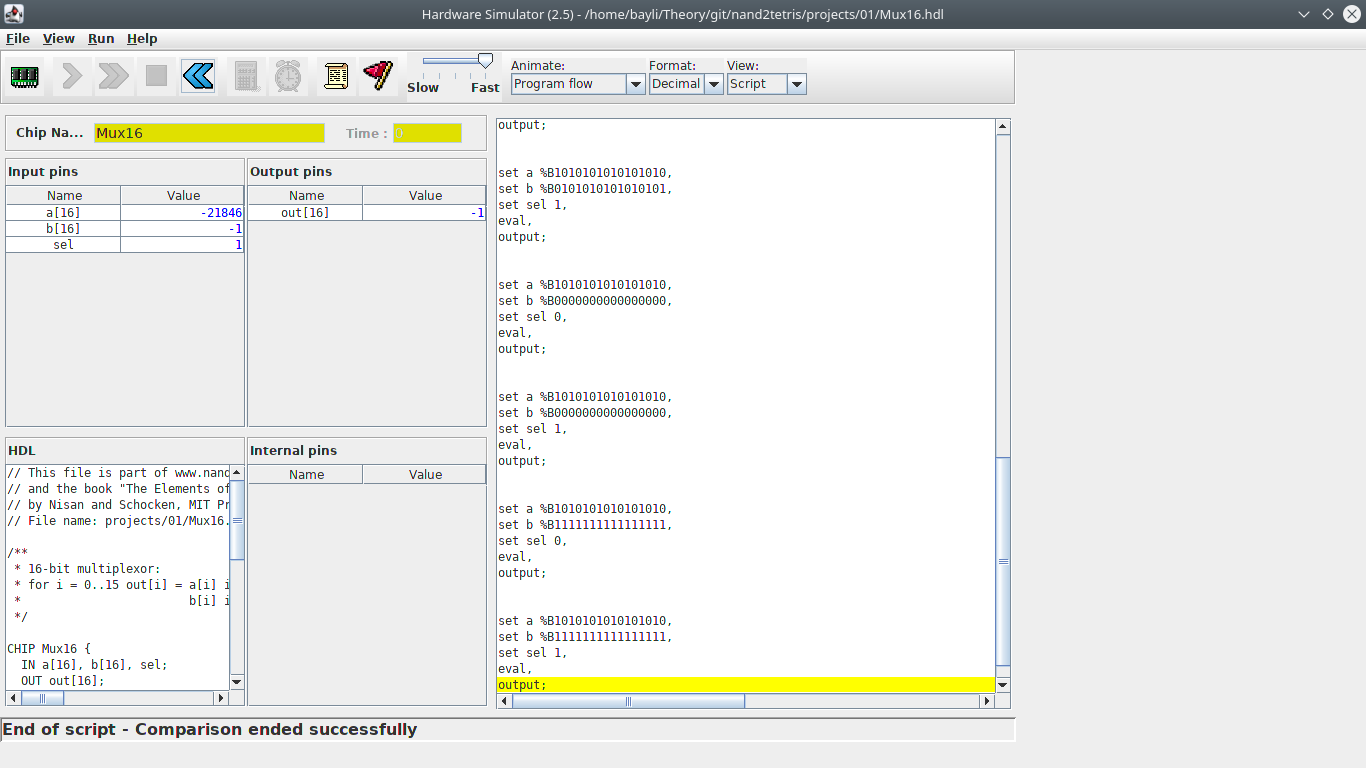
\includegraphics[width=.9\textwidth]{01/Mux16.png}
  }
  \item[Not]{
    All test passed

    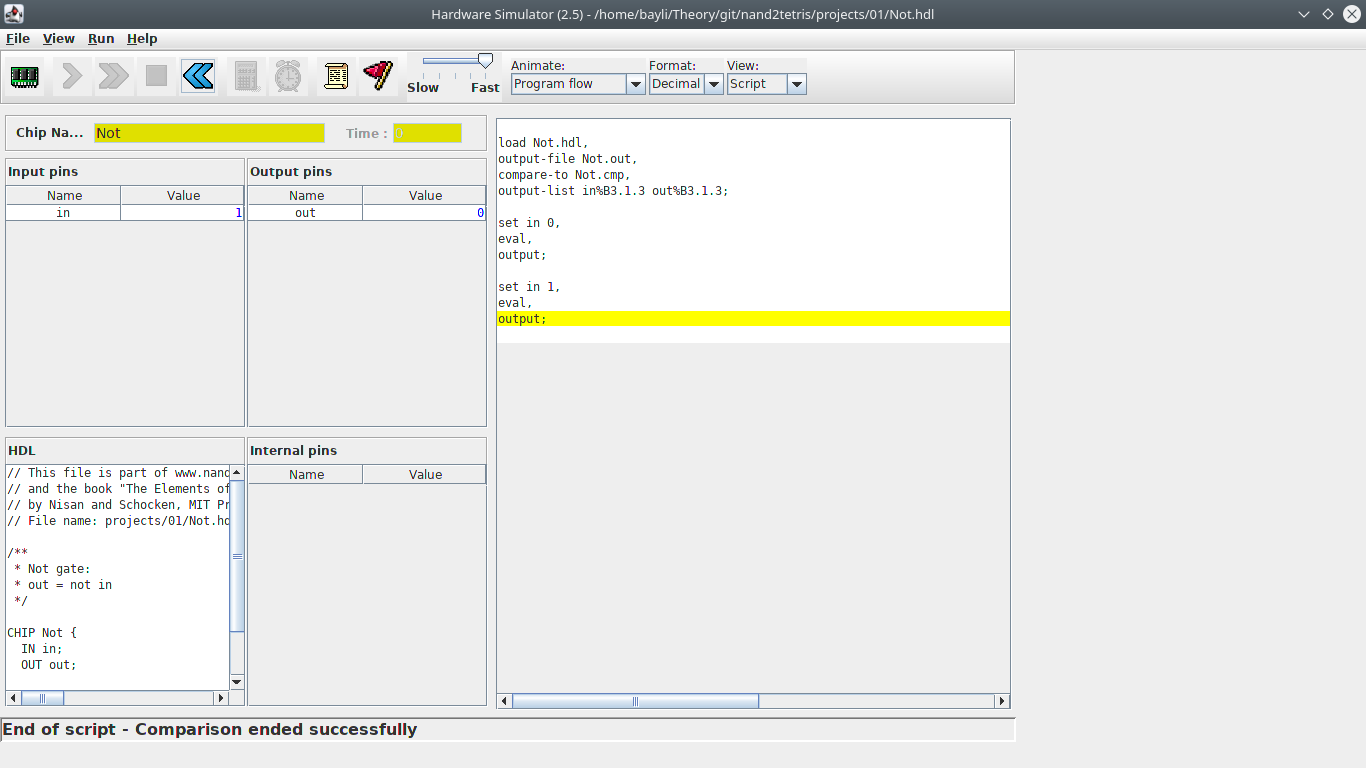
\includegraphics[width=.9\textwidth]{01/Not.png}
  }
  \item[Not16]{
    All test passed

    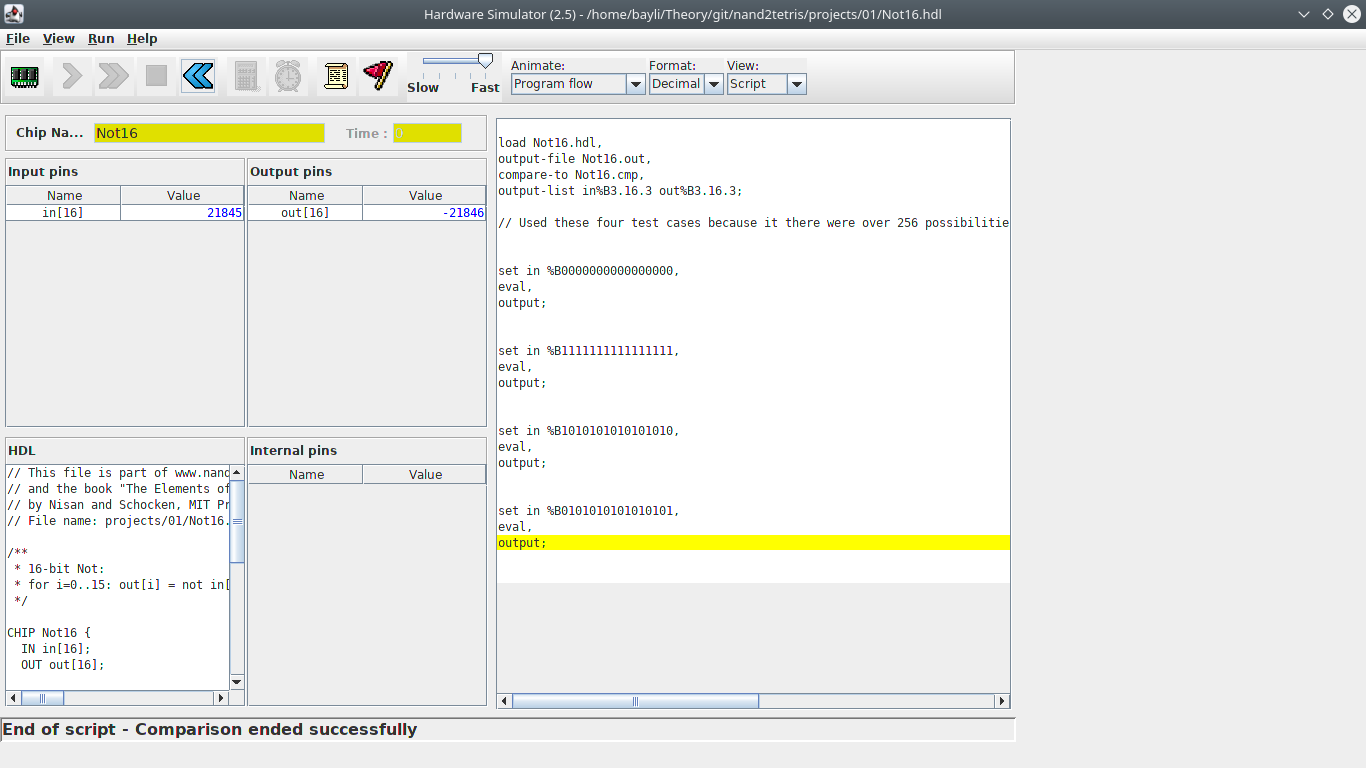
\includegraphics[width=.9\textwidth]{01/Not16.png}
  }
  \item[Or]{
    All test passed

    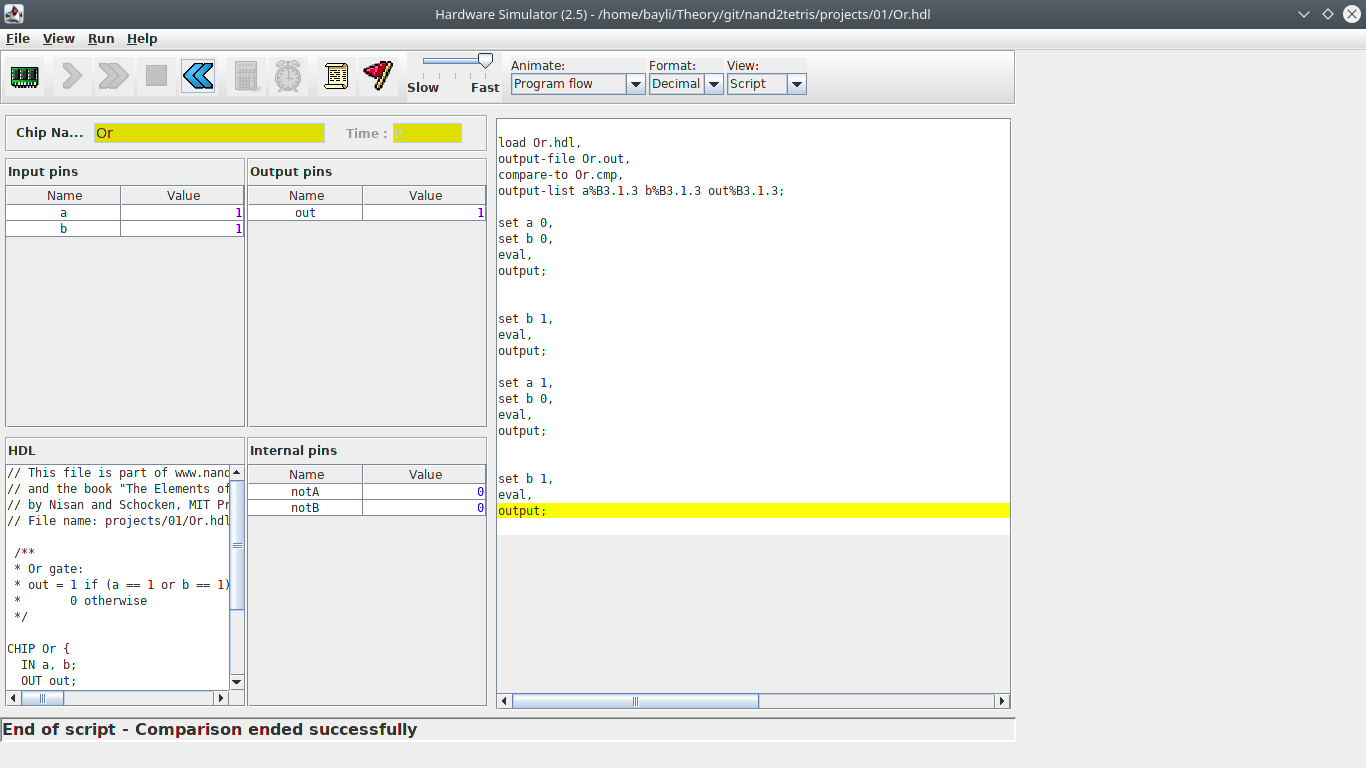
\includegraphics[width=.9\textwidth]{01/Or.png}
  }
  \item[Or8Way]{
    All test passed

    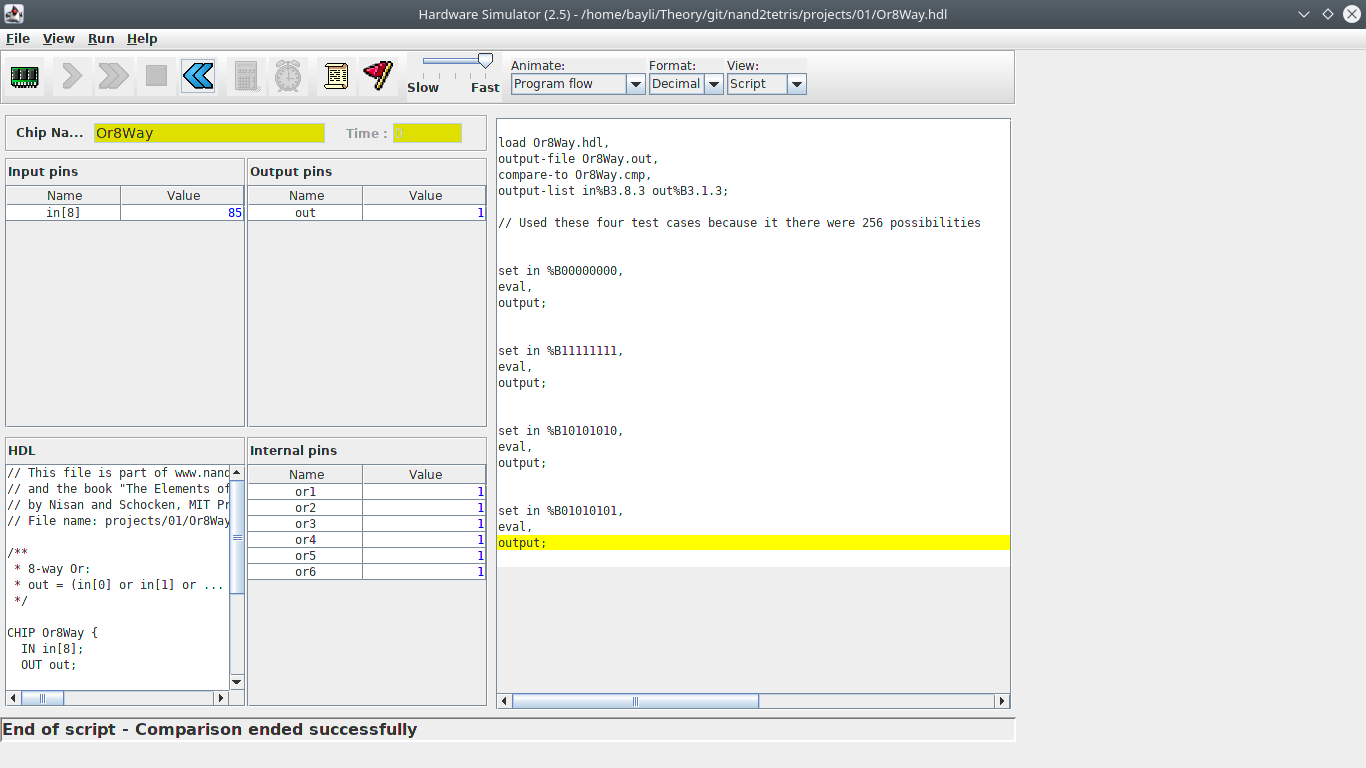
\includegraphics[width=.9\textwidth]{01/Or8Way.png}
  }
  \item[Or16]{
    All test passed

    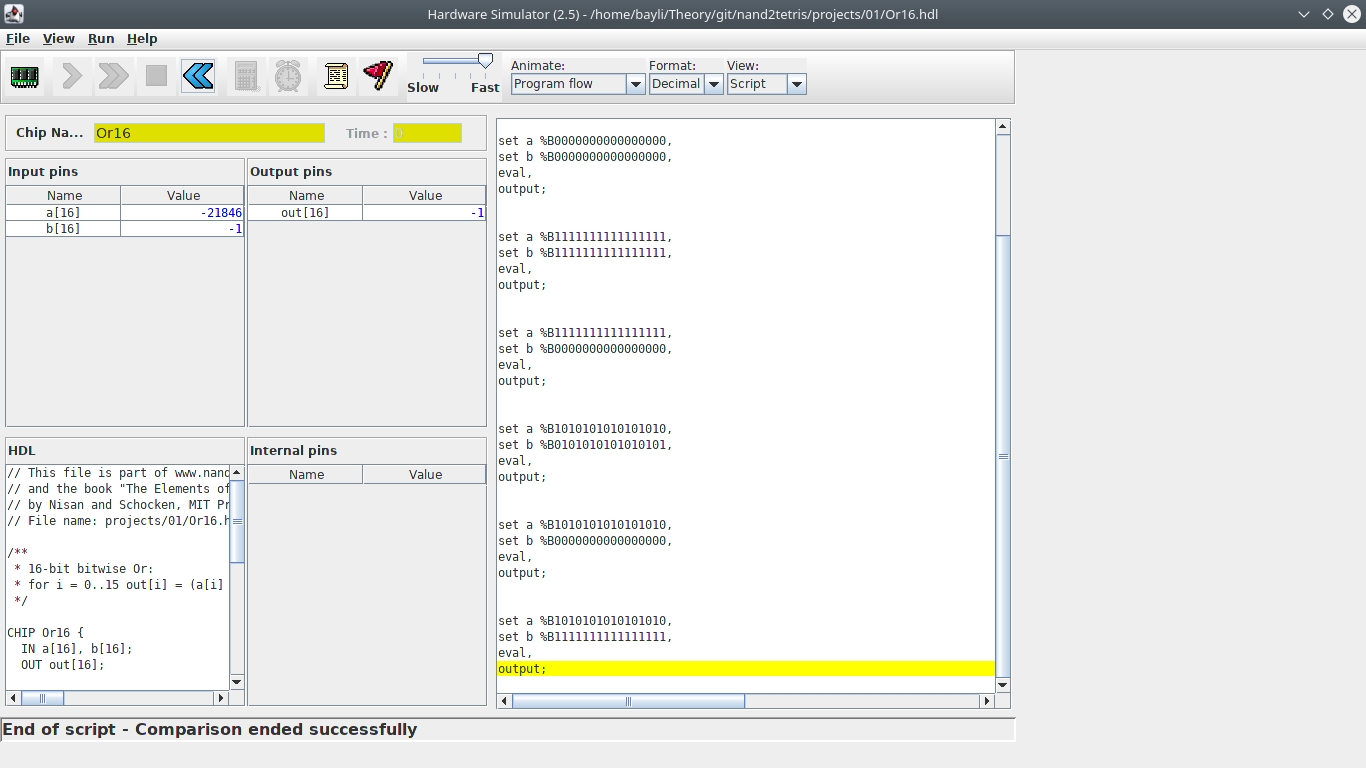
\includegraphics[width=.9\textwidth]{01/Or16.png}
  }
  \item[Xor]{
    All test passed

    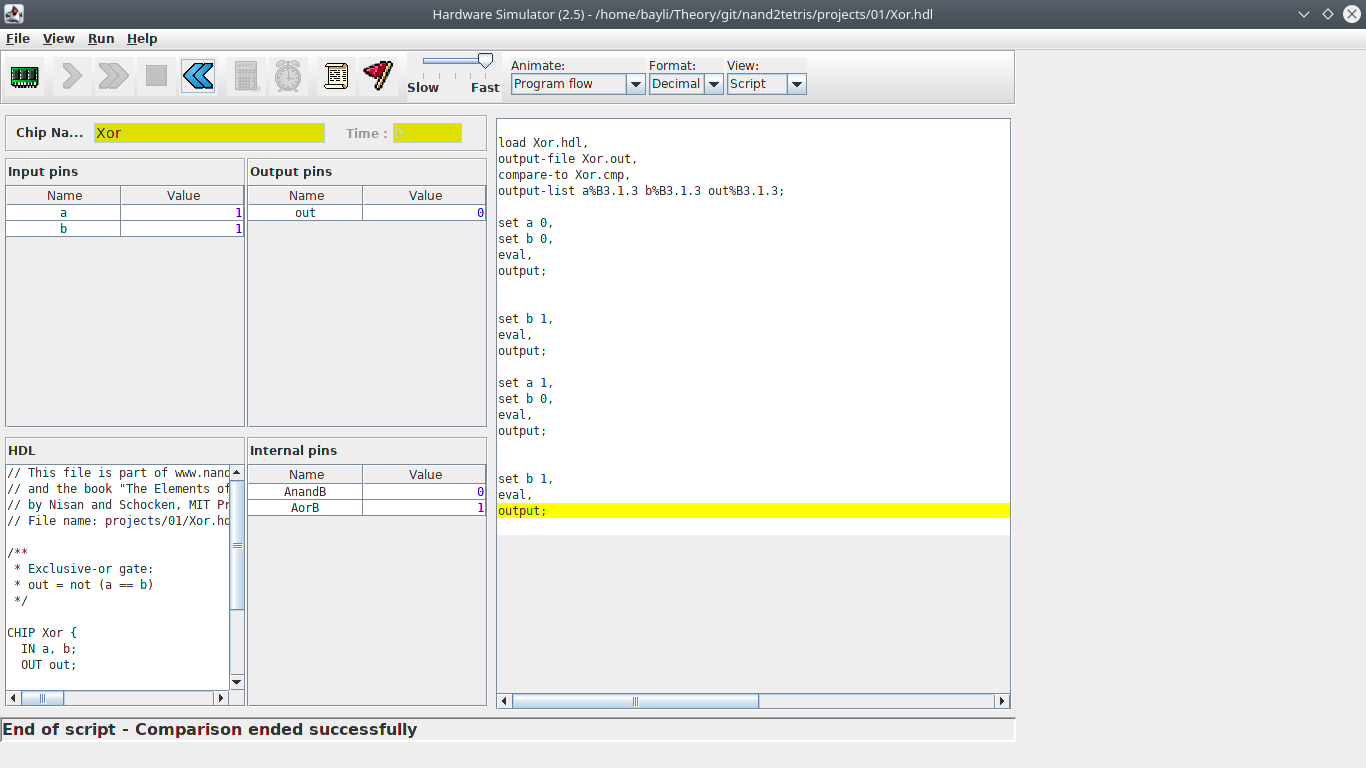
\includegraphics[width=.9\textwidth]{01/Xor.png}
  }
\end{description}

\section{Project 2}

\begin{description}
  \item[Add16]{
    All test passed

    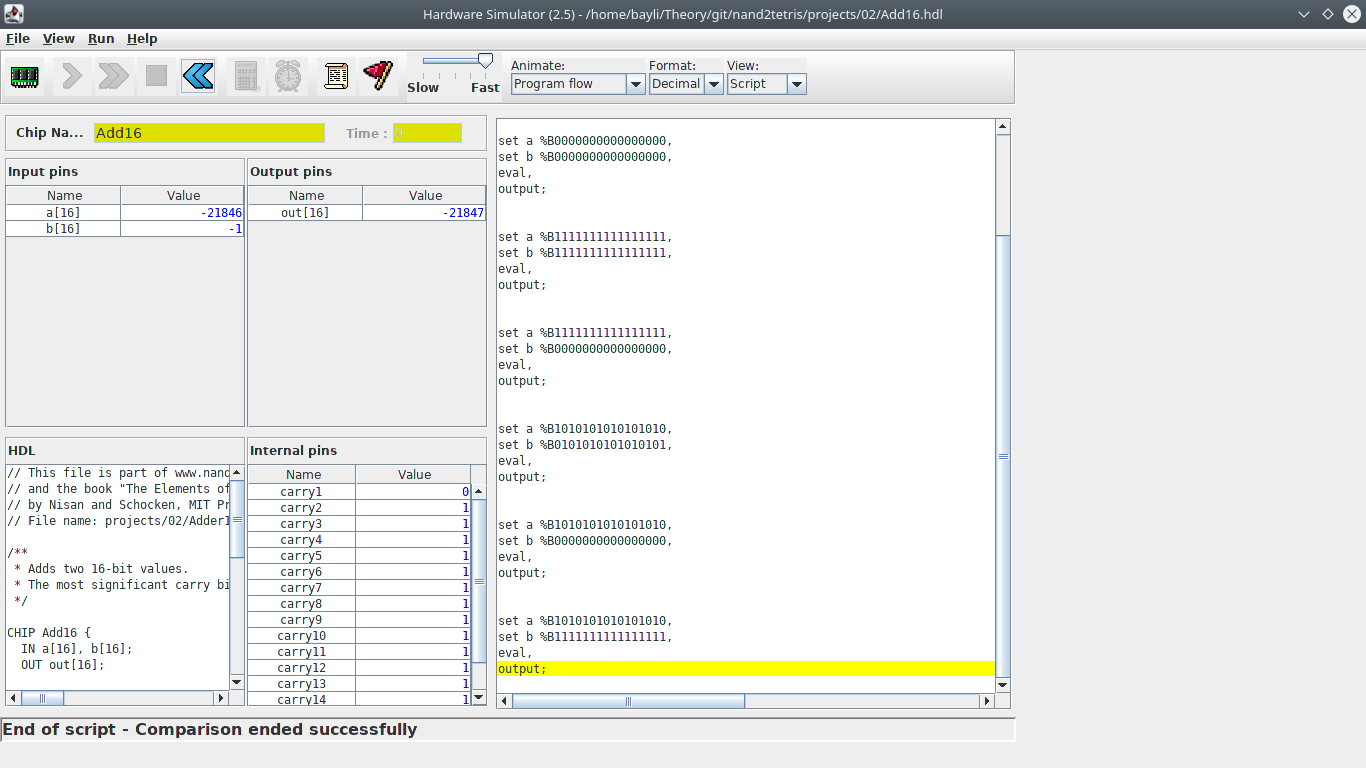
\includegraphics[width=.9\textwidth]{02/Add16.png}
  }
  \item[ALU]{
    All test passed

    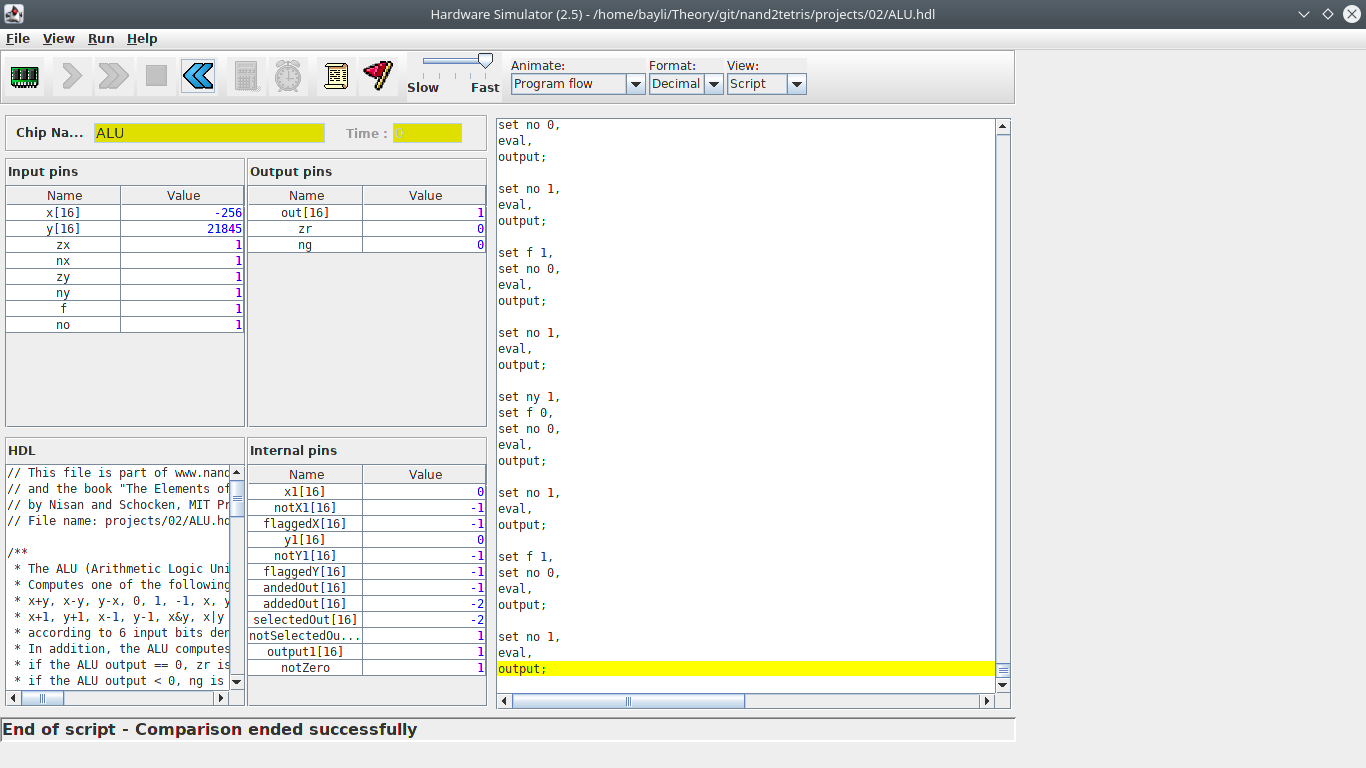
\includegraphics[width=.9\textwidth]{02/ALU.png}
  }
  \item[FullAdder]{
    All test passed

    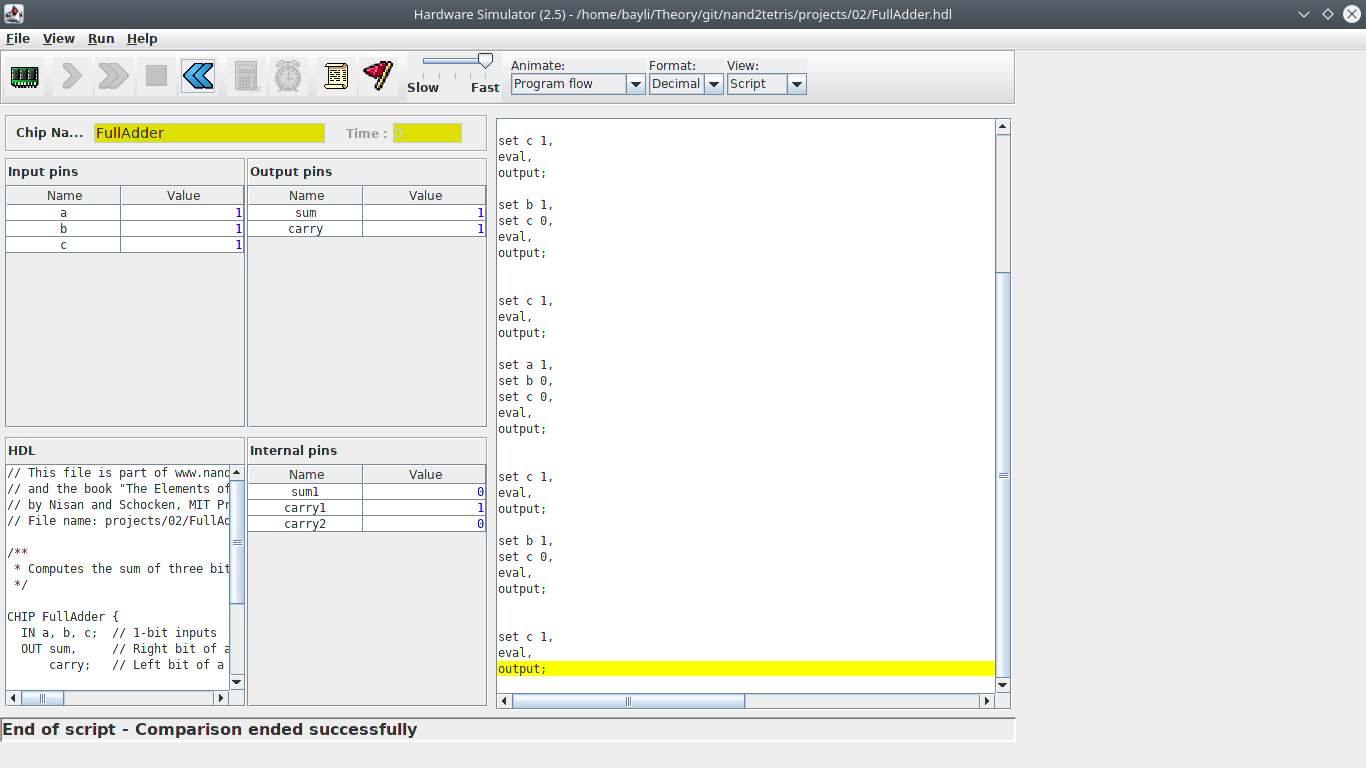
\includegraphics[width=.9\textwidth]{02/FullAdder.png}
  }
  \item[HalfAdder]{
    All test passed

    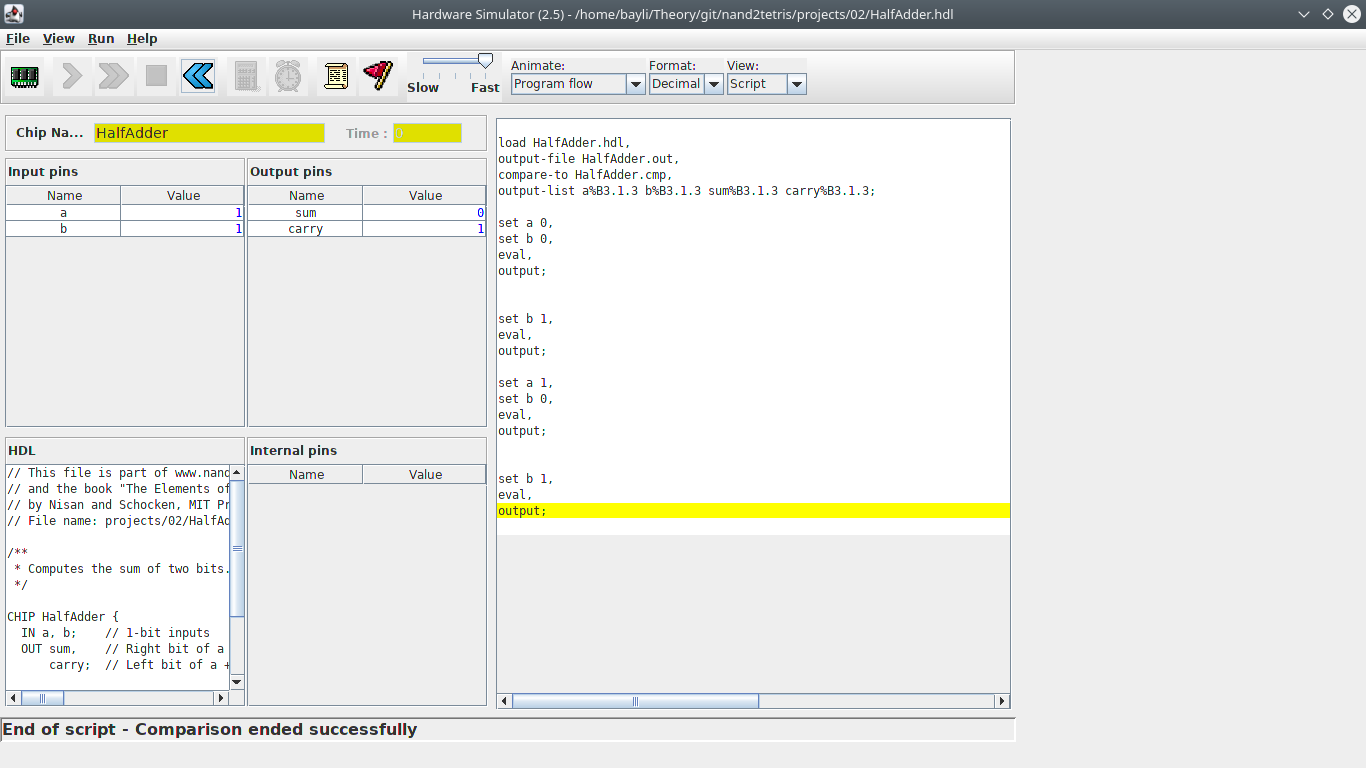
\includegraphics[width=.9\textwidth]{02/HalfAdder.png}
  }
  \item[Inc16]{
    All test passed

    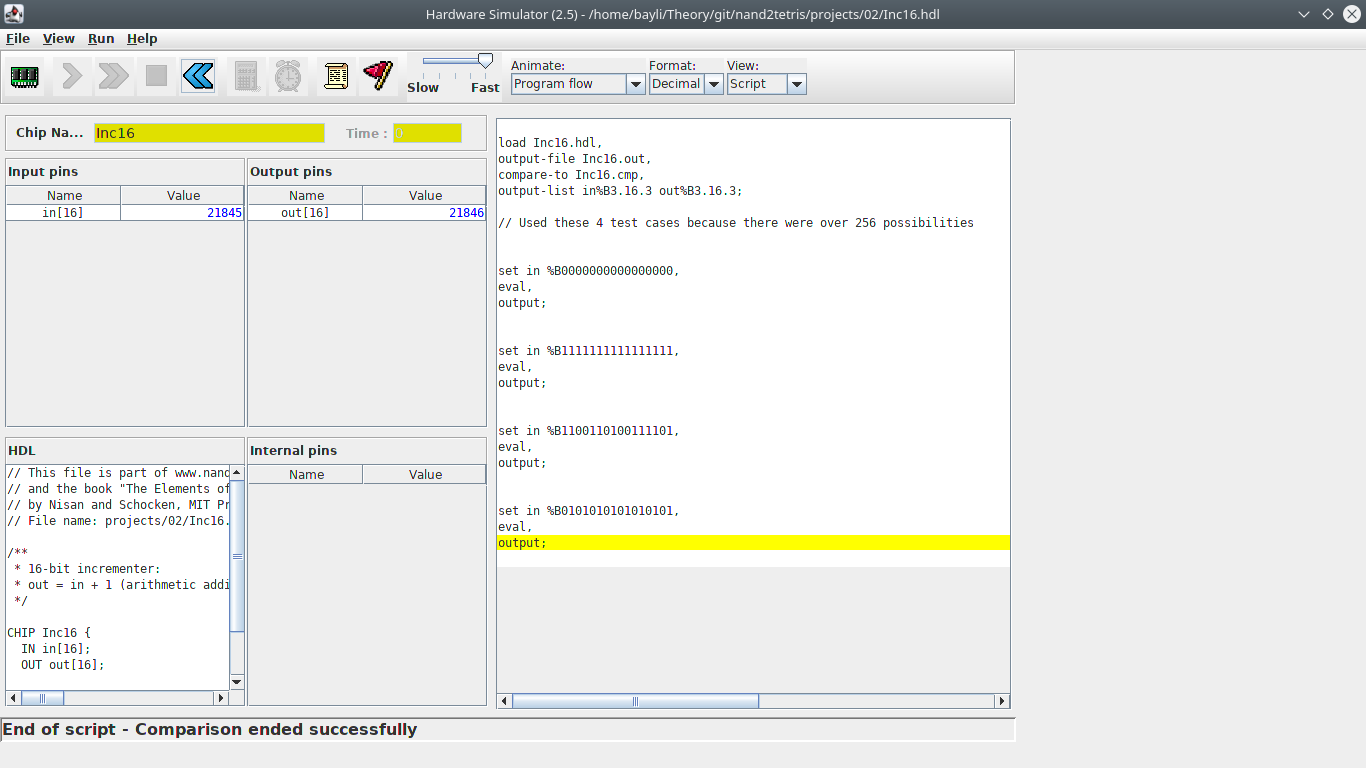
\includegraphics[width=.9\textwidth]{02/Inc16.png}
  }
  \item[Or16Way]{
    All test passed

    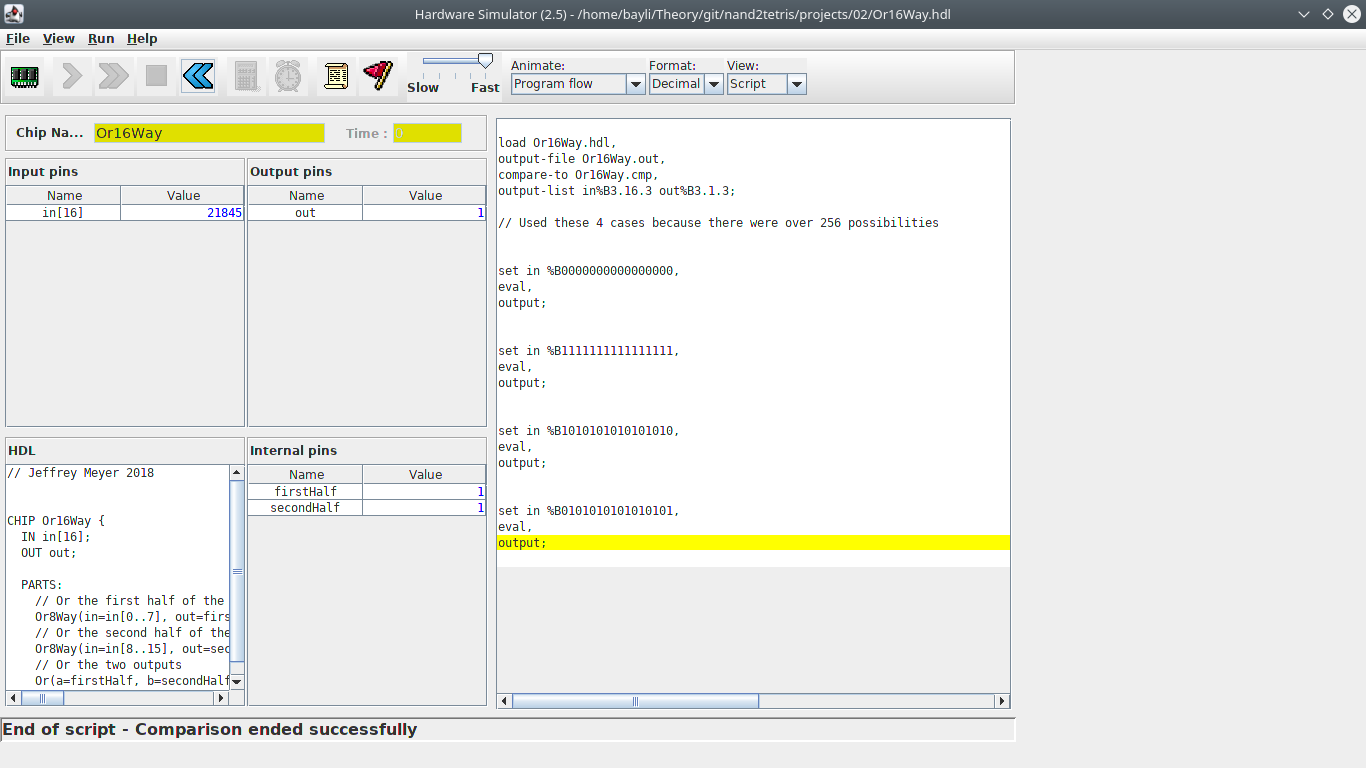
\includegraphics[width=.9\textwidth]{02/Or16Way.png}
  }
\end{description}

\section{Question 3}

\begin{enumerate}[label=(\alph*)]
  \item{
    The ALU has 6 bit flags and 2 16 bit inputs in total giving

    $$2^6 \times 2^16 \times 2^16 = 274,877,906,944$$
  }
  \item{
    There are 36 test cases in the original test file.
  }
  \item{
    For our version of the no-stat test file, we ended up with 641 test cases.
    We decided the flags were the largest likely source of error and to
    exhaustively test each flag with only a few edge case inputs.
  }
  \item{
    The no-stat ALU is the same without the need to compare output cases for if
    the output is negative or zero.  So $274,877,906,944$
  }
  \item{
    There are 36 test cases provided.
  }
  \item{
    The same as the no-stat file, we decided to exhaustively test all the flags
    with a few inputs.
  }
\end{enumerate}

\end{document}